\documentclass{article}
\usepackage{a4wide}
\usepackage{graphicx}


%% if your are not using LaTeX2e use instead
%% \documentstyle[bnaic]{article}

%% begin document with title, author and affiliations

\title{Distributed Computing Systems IN4391\\ The Dragons Arena System %: Distributed Simulation of Virtual Worlds
}
\author{Patrick Brand (p.brand@student.tudelft.nl) \and
    Raies Saboerali (r.a.a.saboerali@student.tudelft.nl)
	%\thanks	T.A: Ir. Mihai Capota, Course Manager: Dr.ir. Alexandru IOSUP
}
\date{}

%support cast needs to be filled in here.


\pagestyle{empty}

\begin{document}
\maketitle
\thispagestyle{empty}

\begin{abstract}
%a description of the problem, system description, analysis overview, and one main result. Size: one paragraph with at most 150 words.
This report discusses the the process of implementing a distributed version of the Dragon Arena System (DAS) in order to be scalable and to support multiple concurrent users playing the game.
The game architecture will consist of two main layers; the helper server layer and the main server layer.
The helper servers will perform computation and the servers in the main layer will keep track of the battlefield en eventual copies of the battlefield.
The communication between the servers and the clients and servers will be done via Java's Remote Method Invocation.
\end{abstract}


\section{Introduction}

%(recommended size, including points 1 and 2: 1 page): describe the problem, the existing systems and/or tools about which you know (related work), the system you are about to implement, and the structure of the remainder of the article. Use one short paragraph for each.
The Dragon Arena System (DAS) is an online warfare game of WantGame BV.
WantGame BV wants to implement a distributed version of the DAS in order to be able to support multiple concurrent users and make the system scalable.
The game will be implemented in Java and will use Remote Method Invocation (RMI) in order to support remote call to other servers.

This report will first discuss a bit about the application itself and its background.
Afterwards, the design and architecture of the proposed system which is going to be implemented will be discussed. 
The various high level components of the game and how they communicate will be explained.
In the third section the results of the various performed tests are presented and at last there will be a discussion about the findings of our work.

\newpage

\section{Background on Application }

\section{System Design}
This section will first discuss how the system operates, by describing how the distributed game engine will operate.
After this, the fault-tolerance will be discussed and at last the scalability components of the system.

\subsection{System Operation}
The general setup of the DAS system consists of Master Servers, Helper Servers, Backup Servers, and Clients.
To initialize the game, one instance of the master server needs to be started. 
The master server will then contain the battlefield and a list of units playing on the battlefield.
The battlefield on this master server only contains a limited set of actions which can be performed.
The actual computation of these actions will not be be computed on the main server, but instead these will be computed on the helper servers.
Therefore for the game to function, it is important to also initialize at least one helper server. 
Every time a helper server is initiated, it also registers itself on the main server.
If a user starts the game on his computer, the clients then connects to main server requesting to join the game.
The master server then randomly selects a helper server from the list of his helpers servers.
The necessary details about the lucky helpers server is then returned to the client. 
The client then connects to this helper server and registers itself.
The client also requests the battlefield itself in order to be able to make the correct decisions. 
If everything works well: the user is ready to play!
When a user tries to perform an action, the action is sent to a helper server.
The helper server will then receive the request and, depending on the type of action, the helper will request the required information from the main server.
When this information is received, the helper performs the required computation on behalf of the player and sends the results to the main server.
The server than send a message back to the client in order to inform him about the result of the action.

\begin{figure}[ht]
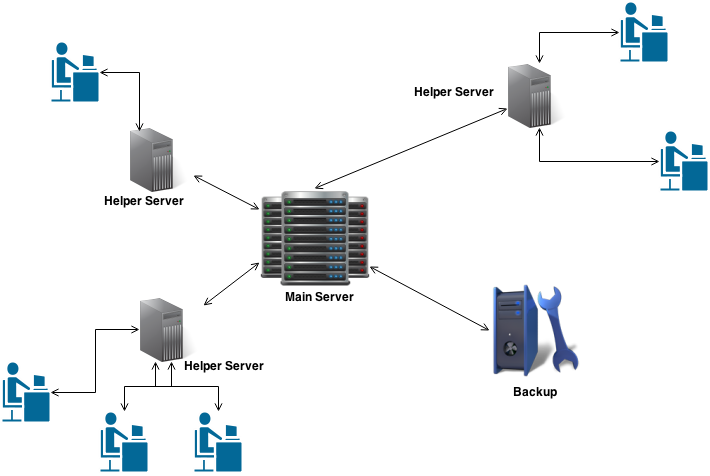
\includegraphics[scale=0.5]{DCS.png}
\end{figure}

\subsection{Fault Tolerance}
Every distributed system is prone to faults, and the Dragon Arena system is not an exception. 
First, lets have a look at the helper servers. As stated earlier, the clients connect to a helper server and register themselves there.
When a helper server goes down, the main server notices this and removes this helper from its known helpers.
If a client tries to query the helper server when it wants to perform an action, it will detect that the helper server is down.
The client then asks the main server for a new helper server.
After the main server updates the client of his new helper, the client registers with the new helper and tries to execute its last action again.
The new helper receives the action request and continues working as usual.

It is also possible that the main server goes down. 
The main server was the one containing the data about the battlefield and its participants.
This is why it is necessary to have a backup server running.  
In order to recover when a main server crashes, the system does check-pointing periodically.
If during the periodic check, the main server detects that there has been changes to the battlefield, the main server sends the changes to the backup server.
The backup server then updates the knowledge of its backup battlefield and other relevant information.

If the main server goes down, it becomes impossible for the helper server to perform any action on the main server obviously.
If the helpers detect such a problem, they immediately try to send the request to the backup server and ask the backup server to perform the action requested on the battlefield.
The helpers also notify the backup, the failure of the main server and tell the main server that he needs to take over the tasks.
Whenever the backup server gets such a notification, it promotes itself to being the main server and takes all the responsibilities of a main server on itself.
The backup may be a few steps behind, because the backup is not made after each Unit action, but periodically. 
Updating the backup after each Unit action would cause too much overhead at the server. 

One problem that can occur is that, when the main server goes down and the backup takes over his work, no other backup server is created. 
If the new main server were to go down, no other server would be able to take over and the game would be lost. 
A solution would be to bring up a new backup server when the new main server is up and running, however attempts to implement this have not proven to be succesful as of yet.

\subsection{Scalability}
In order to support a large number of players on the battlefield, it is important for the system to be scalable.
As stated earlier, the helper servers are performing the computation for the main server.
It is possible to add as many helper servers as required which can be registered to the main server.
Clients may then connect to any of these available helper servers in order to play the game. One of the downsides of doing this is that; the more clients that are connected, the more helper servers you will need which might eventually flood the main server with requests. Another possible downside is; if one decides to spawn less helper servers, for example in order to prevent the previously described problem, one could put too many clients on a helper server, hence stressing the helper servers too much, which might make them unresponsive.

The main server on the other hand, is not scalable for distributing workload like the helper servers do. 
Instead, only a backup is created of the main server, which can be used if the main crashes.
Since the helper servers are the ones doing the computation, it is also not necessary for the main server to have multiple instances for distributing the workload.
 


\section{Experimental Results}
Unfortunately we were not able to utilize the DAS-4 system (due to an incompatible java version), however we tested the game when running on two different laptops over a local area network (LAN). These tests were after the initial deadline and therefore the testing part of the game had already been done. Therefore we decided to spend this chapter on how we wish we could have performed the experiments in the first place if these implementation problems hadn't delayed us this much. However we were able to collect some primitive data from some local experiments. These results will be discussed here as well.

\subsection{Setup}
For this experiment, the DAS-4 should be initialized with 5 compute-nodes. 
One compute node should host the main server which initializes the battlefield. 
Another compute node should initialize the backup for the main server (the backup server). 
Another 2 nodes should be used as the helper servers which connect to the main server. 
Finally the last node can be used to instantiate 3 clients which connect to the randomly distributed helper server nodes.

\subsection{Consistency Experiments}
The purpose of causal consistency is to make sure that events that are causally related are actually ordered. 
To measure this, it is necessary to assign a timestamp upon message creation. 
Additionally, each message is provided with its own unique identifier. 
Every message which is received should be stored in a list and assigned a timestamp which represents the time of arrival.
Whenever a new message is received, its timestamps should be checked with the other timestamps of messages in the list in order to check causality. If the newly received message was sent before a message which has already been received, and these messages are causally related, then the causality constraint is certainly not met.
In this project, a causal relationship is defined by: a certain unit \emph{A} performs an action which has an effect on the state of a certain unit \emph{B}, for instance if a player \emph{A} attacks a dragon \emph{B}.

It is also important to measure how consistent the backup of the battlefield is with the battlefield on the main server.
This can be measured by taking a snapshot of the battlefield on the main server at a random time after which the main server is forcefully shut down. 
At this moment, the taken snapshot can be compared with the latest backup of the battlefield at the backup server. 
The difference in location of the units are an indicator of the consistency between the backup and the main server. The difference in healthpoints of the units can be a measure as well. The combination of these two measures will give a rough indication of the divergence of the backup compared to the main server. 
A more concrete measurement can be obtained by backing up the previously mentioned list of messages and checking the differences between both battlefields. The amount of missing messages in the backup is the exact number of events that were lost during the recovery, hence a clear indication of the inconsistency. 
This experiment should be performed several times in order to guarantee an unbiased result, as the random time of the snapshot will probably sample at different times after the creation of the latest backup at the backup server. 

\subsection{Scalability and Performance Experiments}
In order to test scalability it is important how scalable the helper servers are and how scalable the main server is. 
First, to test the scalability of the helper servers, it is important to have just one variable in this test environment. 
The variable for the scalability of the helper server test lies in the amount of connected clients. 
Therefore we have one fixed main server and one helper server.
The number of connected clients are increased per test run. 
During the tests, the system of the helper server is monitored.
Just like in the previous section, the messages and their timestamp are also recorded.
For each test run, the average response time can be computed.
Then, these response times can be compared which each other in order to check if an increase in clients has an impact on the response time of the server.
If the response time dramatically increases, it is clear that the system is limited to the number of clients it can scale to. 
This is also an indicator for the performance of the system.
The memory and CPU usage should also be recorded  and compared with each other for each test run in order to find the performance bottleneck. 
The only constraint is, that the same hardware is used during every test run.

It is also important to test how scalable the main server is. 
As already stated, there is only one main server active, but the number of helper servers may be increased.
This test will measure  the number of helper servers the main server can handle.
The number of clients per helper server will be kept consistent for each test in this experiment, only the number of helper servers will be increased for each following test run.
The same properties as in the scalability of the helper servers will be measured, but now for the main server.
Instead of measuring the response time of messages between helper and client, the response time between helper and main server is measured.
The CPU and memory usage are also recorded in order to find the performance bottleneck.


\subsection{Fault-Tolerance Experiments}
For fault tolerance the system also needs to be tested for both the helpers and the main server.
To test the tolerance of the system when helpers crash, tests are run with multiple helper servers which are killed at random to simulate crashes.
It is then possible to measure the number of messages which were tried to be sent from the server and the number of messages which were actually sent to a helper server after one was randomly killed.
This tests needs to be run multiple times and the different outcomes should be compared in order to get a view of the number of failed sent messages.
If this value is low, it is probably safe to conclude that the helper server's fault-tolerance is acceptable.

The same experiment should be done for measuring the tolerance of the main server.
Instead of killing a helper, the main server should be killed, and then the backup server should take over the responsibilities of the main server.
During this test, the number of missing messages (events) should be measured by taking the difference between the number of messages on the backup server and the main server, just like it is explained in the section about the scalability.
Also, the number of failures after the backup server is promoted to main should be taken into account.
The less failures after the restore, the better the recovery mechanism is.

\subsection{What actually happened}
% Setup
During the implementation of the game, the game was mainly tested on the local machines.
To simulate the distribution of the system locally, different RMI registries were used for the main classes which are supposed to run on different nodes.
By doing so, the running classes need to call a different (local) server in order to make an RMI call.

% Consistency
One important issue in a distributed game is keeping the game-state consistent for every client and server.
This means that battlefield needs to be somehow updated for every client in order to be able to play the game.
As stated in the previous chapter, the whenever a client sends a request, the required information is returned to the helper server the client is connected to.
The helpers server itself does not maintain a local state of the game, but only computes results.
However, the battlefield does maintain a state of the game. 
Therefore it is important for the master server to maintain a correct state of the game, which is done by sending messages whenever a Unit performs an action and also when certain parts of the game state need to be updated.

As stated, the fancy measurements were not performed during this project. 
However, we did collect some results for helpers and the main server.
The number of messages which were sent and received are logged and as well as the number of messages which were failed to send.
These results are from tests in which the system is spawning the players by reading a file from the Game Trace Archive.
No helper nodes were killed.
It is still notable that there are still some messages failing to be sent. However the number of messages which failed is really small.
What is also observed, is that the failures in the helper servers is much lower than the failure in the main server.
This is probably because the main server eventually receives many more requests than each helper server.

For scalability tests we did not collect hard evidence. 
However, there we did run some tests in which random helper servers were killed after which the clients reconnected to other helper servers.
The clients were also able to continue playing the game.

Another thing which can be noted from the metrics, is that the nodes are quite balanced.
Even though the helper servers are chosen at random it still shows that every helper node has a fair amount of clients.
During the tests there was no case in which almost all clients were connected to one server node and every other helper was doing almost nothing.
Because these nodes are quite balanced, clients can reconnect faster to other helper nodes, simply because the number of helper nodes which need to reconnect is not large.

In the end we also tested the game on two laptops that were connected through a LAN. Although the game ran, some issues came up which were mainly related to updating the movement of the players. We think this is due to the great amount of messages that the main server needs to handle in a very short time period without any form of buffering.

\section{Discussion}
As stated earlier, the implementation of the game did not progress as planned.
In the beginning of this project, it was decided to have one main server and multiple helper server in order to take off some workload of the main server and in order to minimize the synchronization between servers.
This sounded pretty awesome and doable for the implementation of this game.
However, at a certain point in the implementation it came to our knowledge that this is actually not such a good idea at all.
At least not in this case for the implementation of the Dragon Arena System.

In order for the helper servers to take load of from the main and perform computation on behalf of the main server, the helper servers had to do way more messaging in order to make a single action happen than was expected.
A possible solution for this would be to have multiple servers with battlefield to which users can connect.
The battlefield can then handle the actions of the clients by himself, this would eliminate the need for a helper server, thus eliminating a layer of communication and therefore making the game a bit faster (at least that's what we expect). 
This also means that there needs to be some sort of synchronization between the different main servers.
A possible way to do so: check if the move is possible on all the servers, then lock the area which needs to be updated, and then propagate the update further to other battlefields and release the area.
Another positive side of this solution is that no extra backup server is needed, because there are multiple servers with the same battlefield running which could be used if another server crashes.
As explained in the experimental results, during the last minute tests it became apparant that the messages at the main server where lost. 
This problem probably occured, due to the many messages that the main server had to handle in a short period of time. A possible way for fixing this is by storing the messages before handling them. An option for the storage is for example a database which stores the messages that contain the actions of the players.

The current implementation of the DAS does work, however one big trade-off had to be made in order to let the game function correctly.
As stated earlier, the helper servers where needed in order to perform computation. 
This was causing an action to wait for a lot of messages before actually performing the action.
To reduce this number of messaging, a part of the computation was moved back to the main server.
This made the system less distributed than we actually wanted it to be.

\subsection{The use of a Distributed DAS}
The main question still is, if it is useful for WantGame BV to use a distributed system for the game.
Even though the implementation did not go as planned, the game still performs well under good conditions.
A different architecture as proposed earlier in this section would be better of course, but this does not mean that the current implementation does not work at all.
The system was also tested with a 100 players and 20 dragons and still performed very well.
Also, the number of failures were pretty low and switching between helper servers when one of them failed did not cause any major problems.
However, the system was not tested for a number of players way larger than 100.
So it cannot be said for sure that the game will still perform well with when the number of players is higher than 100.

\subsection{Confession}
In the final implementation of the game, the backup service for the main server had to be disabled (partially).
The backup server is able to run but not keep track of the map and the units. 
When the main server goes down, the backup server will start a clean battlefield instead of a restored version of the battlefield.
In order to support the Dragons to be able to send messages it was made a remote object and registered to the RMI registry on the main servers.
This however caused the backup to fail when trying to backup a spawned Dragon object, because it was bound on the main server.
In order to fix this, a Dragon controller has to be make in order to control a Dragon. 
Then this Dragon controller should have been bound instead of the Dragon object itself, therefore making it possible to backup the Dragon objects.





\section{Conclusion}
The implementation of a distributed game is quite a challenge, certainly if you're a beginner in the Distributed Systems field. 
It is safe to conclude that in this case the helper servers are not of much use and that the use of multiple battlefield servers could have been better.

On the other hand the experiments do show that the current implementation does scale and is able to support multiple concurrent users, although it can be concluded that the current implementation is more client-server oriented rather than fully distributed with at least 5 nodes.

Besides the system being scalable, it is also fault-tolerant up to a certain level as clients may also recover from helper server crashes by just reconnecting to a different one and the main server may be replaced by a backup server if it crashes.
Even though the implementation isn't fully distributed, it does not mean that the current design (regardless of its implementation) is all that bad. 
The idea of relieving the main server of some load would still be a nice feature, especially if the computations of the game would have been more resource demanding. 

 \section{Evaluation}
 This section describes our personal experience of the project, where mainly the encountered pitfalls are discussed.

As we experienced, one might easily get tempted to go too much into detail right from the start of the project.
After the written part about \emph{Consistency and Replication}, the first thing we did was focus on the algorithms, for implementing \emph{causal consistency} for instance. 
At some point we came to the conclusion that this took too much time if we wished to follow this approach for all our design choices, hence we started looking for libraries that could provide us with an implementation. 
In the end, it was clear that this should not be the focus of the project and therefore an initial (primitive) distributed concept was designed and eventually implemented. 
Unfortunately this costed us a lot of time that is not represented in the final results (e.g. this paper and the implementation of the system).

Another problem that we faced was our decision of refactoring the given codebase. 
A lot of time was spent on trying to make the given code work, instead of developing a new system from scratch while keeping the given implementation as a valuable resource in mind.
In the future we would start with designing a basic concept and simply implement that concept. After the basic functionality, like for example game logic, would run, we would expand our horizon and look at the more advanced topics in order to improve the system. These topics might include constraints for consistency, scalability and performance for instance.
With this approach it is very likely that the initial design has to be revised when the more advanced topics are implemented, but at least a basic working version can always be retreived by version control.

\section{Open-source}
We have made the code of our DAS game open-source under the BSD new license.
Our code is avaiable on: \url{https://github.com/pbrand/DCS-Dragon-Arena-System} (currently on the development branch)
Link to license: \url{https://github.com/pbrand/DCS-Dragon-Arena-System/blob/development/Game/LICENSE} (currently on the development branch)
  

\section{Appendix}

\subsection{A: Time sheets}

\begin{table}[h]
\begin{tabular}{llllll}
\textbf{Week} & \textbf{think-time} & \textbf{dev-time} & \textbf{xp/analysis-time} & \textbf{write-time} & \textbf{wasted-time} \\ \hline
2             & 2                   & 0                 & 0                         & 0                   & 4                    \\
3             & 3                   & 0                 & 0                         & 2                   & 0                    \\
4             & 3                   & 3                 & 0                         & 0                   & 3                    \\
5             & 1                   & 4                 & 0                         & 0                   & 2                    \\
6             & 1                   & 8                 & 2                         & 3                   & 0                    \\
7             & 1                   & 8                 & 3                         & 2.5                 & 0                    \\
8             & 2                   & 4                 & 4                         & 4                   & 0                    \\
              &                     &                   &                           &                     &                     
\end{tabular}
\end{table}

In the analysis above the hours of the team members are summarized. 
It is clear that in the first two weeks we did not implement anything, but thought more about the system architecture and the possible solutions for the different problems such as consistency and replication.
In the fourth week we started diving in to RMI by reading about RMI and following developer tutorials in order to get familiar with  RMI.
We also started looking in to the provided source code of the DAS system provided on Blackboard and made a start for the implementation.
In the fifth week continued the implementation of the system.
In this week most of the problems (which we already explained in the report) were encountered. 
We decided to start a clean implementation again, which is also why our dev-time in the following weeks were quite high.
As explained in the report, we did not have any fancy experiments. 
However, we did test and experiment with the system in other ways as explained.
These tests includes testing the system with a few clients as as well as tests with multiple clients and helpers performing multiple concurrent actions.
The time we spend doing so is reported under xp/analysis-time.

NOTE: this table is per person, and the total amount of hours in this table is 67.
Which means that the total for all the members is twice this number.
The amount of hours spent by each member is almost the same, which is why we just provided one table.
This is mainly because we scheduled meetings to work on the assignment.

\subsection{B: Evaluation}

 \section{Evaluation}
 This section describes our personal experience of the project, where mainly the encountered pitfalls are discussed.

As we experienced, one might easily get tempted to go too much into detail right from the start of the project.
After the written part about \emph{Consistency and Replication}, the first thing we did was focus on the algorithms, for implementing \emph{causal consistency} for instance. 
At some point we came to the conclusion that this took too much time if we wished to follow this approach for all our design choices, hence we started looking for libraries that could provide us with an implementation. 
In the end, it was clear that this should not be the focus of the project and therefore an initial (primitive) distributed concept was designed and eventually implemented. 
Unfortunately this costed us a lot of time that is not represented in the final results (e.g. this paper and the implementation of the system).

Another problem that we faced was our decision of refactoring the given codebase. 
A lot of time was spent on trying to make the given code work, instead of developing a new system from scratch while keeping the given implementation as a valuable resource in mind.
In the future we would start with designing a basic concept and simply implement that concept. After the basic functionality, like for example game logic, would run, we would expand our horizon and look at the more advanced topics in order to improve the system. These topics might include constraints for consistency, scalability and performance for instance.
With this approach it is very likely that the initial design has to be revised when the more advanced topics are implemented, but at least a basic working version can always be retreived by version control.






\nocite{*}
\bibliographystyle{plain}
\bibliography{mybibfile}

\end{document}








